\section{Evaluation}
\label{sec:pytheas:eval}


To evaluate \name, we run our prototype~\cite{ddn-source} across
multiple instances in CloudLab~\cite{cloudlab}.  Each instance is a physical
machine that has 8 cores (2.4 GHz) and 64GB RAM.  These instances are grouped 
 to form two frontend clusters and one backend
cluster (each includes 5 to 35 instances).  
This testbed is an end-to-end implementation of \name described in
Section~\ref{sec:pytheas:impl}\footnote{\name can use standard solutions such as DNS redirection
to map clients to frontend clusters, and existing load balancing mechanisms provided by the host
cloud service to select a frontend server instance for each client.}.


By running trace-driven evaluation and microbenchmarks on this testbed deployment, we show that:
\begin{packeditemize}
\item In the use case of video streaming, Pytheas improves the mean QoE by up to 6-31\% and the 90th percentile QoE by 24-78\%,
compared to a prediction-based baseline (Section~\ref{sec:eval:usecase}).  
\item \name is horizontally scalable and has similar low response delay to existing prediction-based systems  (Section~\ref{sec:eval:scale}).
\item \name can tolerate failures on frontend clusters by letting  clients fall back to local logic and rapidly recovering lost states from
 other frontends (Section~\ref{sec:eval:fail}).
\end{packeditemize}



%\myparatight{Micro-benchmark of performance}


\subsection{End-to-End Evaluation}
\label{sec:eval:usecase}

\mypara{Methodology}
To demonstrate the benefit of \name on improving QoE, we use a real-world trace of 8.5 million video sessions collected from a major video streaming sites in US over a 24-hour period. Each video session can choose one of two CDNs.
The sessions are replayed in the same chronological order as in the trace.
%, thereby allowing \name to gain knowledge as it goes along using newer QoE measurement. 
We call a group of sessions a {\em unit} if they match values on AS, city, connection type, player type and content name.\footnote{The notion of unit is used to ensure statistical confidence of QoE evaluation, and is not used in \name.}
 We assume that when a video session is assigned to a CDN, its QoE would be the same to the QoE of a session that is randomly sampled from the same unit who use the same CDN in the same one-minute time window.
For statistical confidence, we focus on the units which have at least 10 sessions on each CDN in each one-minute time windows for at least ten minutes. 
We acknowledge that our trace-driven evaluation has constraints similar to the related work, such as the assumption that QoE in a small time window is relatively stable in each unit (e.g.,~\cite{via}) and a small decision space (e.g.,~\cite{cfa}).

For each video session in the dataset, we run a DASH.js video player~\cite{dashjs}, which communicates with \name using the API described in Figure~\ref{fig:impl-api}. To estimate the QoE of a video session, the video player does not stream video content from the selected CDN. Instead, it gets the QoE measurement from the dataset as described above.

We use CFA~\cite{cfa} as the prediction-based baseline. It is implemented based on~\cite{cfa}.
CFA updates QoE prediction in the backend every minute, 
and trains critical features every hour.  
The frontend clusters run a simple decision-making algorithm -- for 90\% sessions,
it picks the decision that has the best predicted QoE, and for
the rest sessions, it randomly assigns them to a CDN.

We consider two widely used video QoE metrics~\cite{sigcomm11conviva,cfa}: join time (the start-up delay of a video session), and buffering ratio (the fraction of session duration spent on rebuffering).
 We define improvement of \name for a particular unit at $t$-th minute by
  $\mathit{Improve}_{\mathit{\name}}(t)=\frac{Q_{CFA}(t)-Q_{\mathit{\name}}(t)}{Q_{CFA}(t)}$, where $Q_{\mathit{\name}}(t)$ and $Q_{CFA}(t)$ are the average QoE of \name in $t$-th minute and that of the baseline, respectively. 
Since we prefer smaller values on both metrics, a positive 
 value means  \name has better QoE.
%To highlight \name's improvement over the baseline in different units, 
%we define the mean improvement of \name for a unit by $\frac{1}{T}\sum_{t=1}^{T}\frac{Q_{CFA}(t)-Q_{Polis}(t)}{Q_{CFA}(t)}$, 
%Similarly, we can define 90 percentile improvement of each unit.
%In the rest of the section, we consider the \name improvement in these two metrics.


\begin{figure}[t!]
\captionsetup[subfigure]{justification=centering,farskip=-1pt,captionskip=5pt}
\centering
%\hspace{-0.5cm}
\subfloat[Join time]
{
        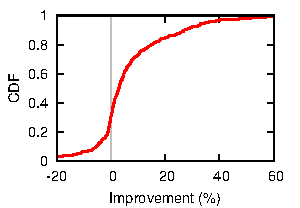
\includegraphics[width=0.45\textwidth]{figures/pytheas-Eval-overall-quality-shijie-2-jointime-cdf.pdf}
	\label{fig:eval-overall-quality-jointime}
}
%\hspace{-0.4cm}
\subfloat[Buffering ratio]
{
        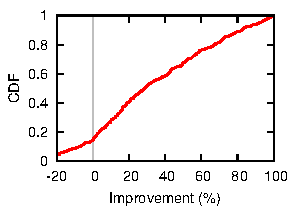
\includegraphics[width=0.45\textwidth]{figures/pytheas-Eval-overall-quality-shijie-2-bufratio-cdf.pdf}
	\label{fig:eval-overall-quality-bufratio}
}
%\hspace{-0.5cm}
%\vspace{-0.2cm}
\caption{Distribution of improvement of \name over the prediction-based baseline.}
%\vspace{-0.2cm}
\label{fig:eval-overall-quality}
\end{figure}

\mypara{Overall improvement} Figure~\ref{fig:eval-overall-quality} shows
the distribution of improvement of \name across all sessions.  We can see that
the mean improvement is 6\% for join time and 31\% for buffering ratio, and the
90th percentile improvement is 24\% for join time and 78\% for buffering ratio.
To put these numbers in context, prior studies 
show a 1\% decrease in buffering can lead to more than a 3-minute increase 
in expected viewing time~\cite{sigcomm11conviva}.
Note that \name is not better than the baseline on every single 
session, because the \mab process inherently uses a
(dynamic) fraction of traffic to explore suboptimal decisions.
% Next, we evaluate two scenarios where \name has greater improvement.


\begin{figure}[t!]
\captionsetup[subfigure]{justification=centering,farskip=-1pt,captionskip=0pt}
\centering
%\hspace{-0.5cm}
\subfloat[Join time]
{
        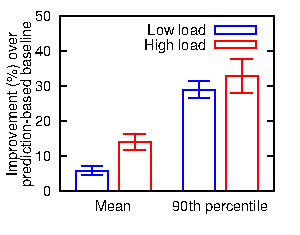
\includegraphics[width=0.45\textwidth]{figures/pytheas-Eval-loadeffect-shijie-jointime-2.pdf}
	\label{fig:eval-loadeffect-jointime}
}
%\hspace{-0.4cm}
\subfloat[Buffering ratio]
{
        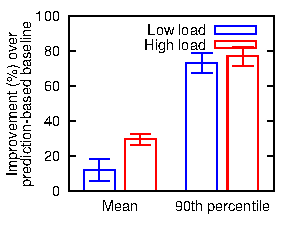
\includegraphics[width=0.45\textwidth]{figures/pytheas-Eval-loadeffect-shijie-bufratio-2.pdf}
	\label{fig:eval-loadeffect-bufratio}
}
%\hspace{-0.5cm}
%\vspace{-0.2cm}
\caption{Improvement in presence of load effect.}
%\vspace{-0.cm}
\label{fig:eval-loadeffect}
\end{figure}

%\begin{figure}[t!]
%\centering
%\includegraphics[width=0.35\textwidth]{figures/motivation/Eval-loadeffect.pdf}
%\vspace{-0.2cm}
%\tightcaption{Impact of load effect on the improvement of \name}
%\label{fig:eval-loadeffect}
%\end{figure}

\mypara{Impact of load-induced QoE degradation}
%We also want to understand the impact of load effect on the benefit of \name.
%To that end, we consider the units whose sessions could have significantly degraded quality when one CDN has a load over certain threshold.
We consider the units where QoE of a CDN could significantly degrade when most sessions of the unit are assigned to use the same CDN.
We assume that the QoE of a session when using a CDN under a given load (defined by the number of sessions assigned to the CDN in one minute) is the same to the QoE of a session randomly chosen in the dataset which uses the same CDN when the CDN is under a similar load. 
Figure~\ref{fig:eval-loadeffect} shows that the improvement of \name when the number of sessions is large enough to overload a CDN is greater than the improvement when the number of sessions is not large enough to overload any CDN.
%We can see that \name has a greater improvement when load-induced QoE degradation is possible. 
This is because the prediction-based baseline could overload a CDN when too many sessions are assigned to the same CDN before CFA updates the QoE prediction, whereas \name avoids overloading CDNs by updating its decisions in real time.

%\cameraremove{\myparatight{Handling flashcrowd}}
%\cameraremove{Finally, we consider when flashcrowd can lead to QoE degradation on certain video object.
%Since this is a VoD dataset, flashcrowd is relatively rare. 
%So we created synthetic trace by adding many video sessions who join at the same moment to watch certain object so that it creates load-induced QoE degradation on CDNs' performance on this particular object.
%Figure~\ref{fig:eval-flashcrowd} shows that \name has greater improvement after a flashcrowd happens. 
%This is because \name can regroup based on real-time feedback on workload.
%}
%
%\cameraremove{
%\camera{Finally, we consider a case where the sessions of a certain video object increase dramatically in a very short period of time, which simulates a flash-crowd event.
%To this end, we created a synthetic trace by adding many video sessions at the same moment to watch the same video object, and this sudden increase in load could led to QoE degradation on CDNs' performance on this particular object. 
%We assume that the sessions of this video object is in the same session group, which in real world may require additional logic to ensure (see \Section\ref{sec:discuss}).
%Figure~\ref{fig:eval-flashcrowd} shows that \name achieves better QoE than CFA, because \name can immediately adjust CDN selection to cope with sudden load increase based on real-time feedback, while CFA cannot react fast enough.}
%}

%Finally, \name should also be robust to flashcrowd. 
%Figure~\ref{fig:eval-flashcrowd} shows the behavior of \name in the example of Figure~\ref{subfig:problem-of-slow:flash}. 
%We can see that because \name detects sharp raise in viewership of object X as soon as it appears, it can react by creating a new group for the session watching X and make different decisions independently to other sessions. 


%\cameraremove{
%\begin{figure}[t!]
%\captionsetup[subfigure]{justification=centering,farskip=-1pt,captionskip=0pt}
%\centering
%\hspace{-0.5cm}
%\subfloat[Join time]
%{
%        \includegraphics[width=0.25\textwidth]{figures/motivation/Eval-flashcrowd-shijie-jointime-2.pdf}
%	\label{fig:eval-flashcrowd-jointime}
%}
%\hspace{-0.4cm}
%\subfloat[Buffering ratio]
%{
%        \includegraphics[width=0.25\textwidth]{figures/motivation/Eval-flashcrowd-shijie-bufratio-2.pdf}
%	\label{fig:eval-flashcrowd-bufratio}
%}
%\hspace{-0.5cm}
%\vspace{-0.2cm}
%\tightcaption{Improvement in presence of flash crowd}
%%\vspace{-0.2cm}
%\label{fig:eval-flashcrowd}
%\end{figure}
%}

\mypara{Contribution of \name ideas}
Having shown the overall benefit of \name, we now evaluate the contribution of different components of \name: (1) \mab;
 (2)  real-time update; and  (3) grouping. 
We replace certain pieces of \name by baseline solutions and compare their QoE with \name's QoE.
 Specifically, for (1), we replace the per-group \mab logic by CFA's decision-making logic; 
for (2), we run  \name with  data of one-minute staleness; and for (3), 
 we run the same \mab process over all sessions, rather than on per-group basis.
%three hypothetical baselines, each of which differs to \name only in one aspect and thus highlights the importance of one aspect of \name.
%\begin{packeditemize}
%\item Benefit of ``\mab'' is shown by ``Real-time CFA'' which differs to \name only in that it runs CFA logic, instead of \mab, for per-group control.
%\item Benefit of ``real-time'' is shown by ``Stale \mab'' which differs to  \name only in that it uses data of one minute stale. One can think of it as a centralized way of running \mab by the backend with stale data~\cite{velox-cidr}. 
%\item Benefit of ``grouping'' is shown by ``Global \mab'' which differs to \name in that it runs the same \mab process over all sessions, rather than on per-group base.
%\end{packeditemize
Figure~\ref{fig:eval-separate} shows the improvement of \name over each baseline, and it shows that each of these ideas contributes a nontrivial improvement to \name; about 10-20\% improvement on average QoE and 15-80\% on the 90th percentiles. 

%First, to highlight the benefit of ``\mab'', we compare \name with a hypothetical baseline called {\em real-time CFA}, which differs to \name only in that it runs CFA logic for per-group control.
%Second, to highlight the benefit of ``real-time'', we compare \name with a hypothetical baseline called {\em stale \mab}, which differs 

%%%% prediction -> real-time prediction -> real-time E2
%%%% global stale e2 -> global real-time e2 -> group-based real-time E2

%we consider a hypothetical baseline called {\em real-time CFA}, which updates CFA QoE prediction at the same frequency to \name (i.e., every second)\footnote{Real-time CFA is feasible in \name, but is impractical in the original CFA implementation since it could not update prediction in real time.}. 
%Figure~\ref{fig:eval-separate} compares the mean and tail improvements of real-time CFA and real-time \mab (\name). 
%We can see that the improvement of real-time CFA is great, but real-time \mab has a much larger improvement, especially on the tails. 
%This suggests that both ``real-time'' and ``\mab'' are needed to achieve full potential of data-driven optimization.



\begin{figure}[t!]
\captionsetup[subfigure]{justification=centering,farskip=-1pt,captionskip=0pt}
\centering
%\hspace{-0.5cm}
\subfloat[Join time]
{
        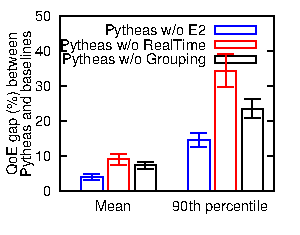
\includegraphics[width=0.45\textwidth]{figures/pytheas-Eval-OtherEE-shijie-jointime-2.pdf}
	\label{fig:eval-separate-jointime}
}
%\hspace{-0.4cm}
\subfloat[Buffering ratio]
{
        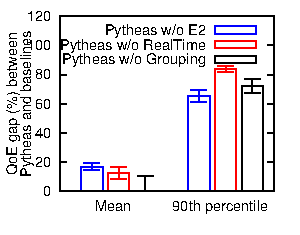
\includegraphics[width=0.45\textwidth]{figures/pytheas-Eval-OtherEE-shijie-bufratio-2.pdf}
	\label{fig:eval-separate-bufratio}
}
%\hspace{-0.5cm}
%\vspace{-0.2cm}
\caption{Factor analysis of \name ideas} %Separating the benefit of ``\mab'', ``real time'', and ``groupping''.}
%\vspace{-0.2cm}
\label{fig:eval-separate}
\end{figure}



\subsection{Microbenchmarks}

\label{sec:eval:scale}

%In addition to the small-scale testbed for trace-driven emulation, 
We create micro-benchmarks to evaluate the scalability and bandwidth
consumption of \name, as well as the benefits of various performance optimizations (Section~\ref{sec:pytheas:impl}).




\subsubsection{Scalability}
\myparatight{Frontend}
Figure~\ref{fig:eval-frontend-scalability} shows the maximum number of sessions that can be served in one second, while keeping the update interval of per-group logic to be one second. 
Each session makes one control request and uploads QoE measurement once. Each group has the same amount of sessions.
The size of control request message is 100B. We run Apache Benchmark~\cite{ab} for 20 times and report the average throughput.
We can see that the throughput is almost horizontally scalable to more frontend server instances. 
%Moreover, \name achieves almost the same throughput to a frontend cluster with the same resource that does not need to run the per-group control logic (e.g., a C3 frontend cluster).
 While  the number of groups does impact the performance of frontend cluster, it is only to a limited extent; throughput of handling 10K groups is about 10\% worse than that of handling one group.

Next, we evaluate the performance optimizations described in Section~\ref{sec:pytheas:impl}.
We use a frontend cluster of 32 instances.
Figure~\ref{fig:eval-optimization-frontend} shows that by separating \mab logic from client-facing servers, we can achieve 8x higher throughput, because each request reads cached decisions, which are still frequently updated.
By replacing features by group identifiers, we can further increase throughput  by 120\%, because we can copy less data from client-facing servers to the servers running \mab logic.
%As a result, the frontend throughput is as high as if all instances are used as web servers without any control logic.
Note these results do not merely show the scalability of Spark Streaming or web servers; they show that our implementation of \name introduces minimal additional cost, and can fully utilize existing data analytics platforms.

%We use one client-facing server instance, and set the request message to be 100B.

%Figure~\ref{fig:eval-optimization-frontend} shows that while unoptimized session-to-group lookup has significantly lower throughput with increasing numbers of groups, block-based lookup can achieve almost the same throughput to a simple web server that does no lookup. 
%Using the same setup, we also found that by separating query of control logic from the process of responding each request, client-facing server throughput is 800\% higher than if each request is processed by querying the control logic (not shown in figure).
%Finally, we increase the request message size, and show in Figure~\ref{fig:eval-optimization-sparkstreaming} that the throughput of per-group logic is very sensitive to the size of session features, and by replacing session features with group identifiers and thus keeping the message size constant, per-group logic can maintain high throughput independently with the message size.


\begin{figure}[t!]
\captionsetup[subfigure]{justification=centering,farskip=-1pt,captionskip=5pt}
\centering
%\hspace{-0.5cm}
\subfloat[Frontend]
{
        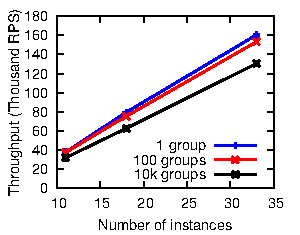
\includegraphics[width=0.45\textwidth]{figures/pytheas-Eval-scalability-frontend.pdf}
	\label{fig:eval-frontend-scalability}
}
%\hspace{-0.4cm}
\subfloat[Backend]
{
        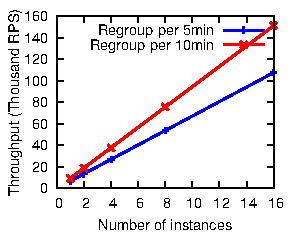
\includegraphics[width=0.45\textwidth]{figures/pytheas-Eval-scalability-backend.pdf}
	\label{fig:eval-backend-scalability}
}
%\hspace{-0.5cm}
%\vspace{-0.1cm}
\caption{\name throughput is horizontally scalable.}
%\vspace{-0.2cm}
\label{fig:scalability}
\end{figure}

\begin{figure}[t!]
\centering
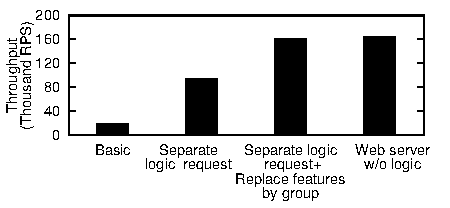
\includegraphics[width=0.6\textwidth]{figures/pytheas-Eval-optimization-separatelogic-replacingfeatures-bar.pdf}
%\vspace{-0.2cm}
\caption{Optimizations of frontend throughput.}
\label{fig:eval-optimization-frontend}
\end{figure}


\mypara{Backend}
Figure~\ref{fig:eval-backend-scalability} shows the maximum number of sessions that can be served in each second by a backend cluster, while keeping the completion time of session-grouping logic within 5 minutes or 10 minutes.
We see that the throughput is also horizontally scalable with more instances in the backend cluster. 

To put the scalability numbers of both frontend and backend in context, let us consider a content provider like YouTube which has 5 billion sessions per day~\cite{youtube-stats} (i.e., 57K sessions per second). 
%. , which is on average 3.5 million sessions per second. 
%the traffic is evenly spread over time, that is 57K sessions per second. 
\name can achieve this throughput using one frontend cluster of 18 instances and a backend cluster of 8 instances, which is a tiny portion compared to the sheer number of video servers (at least on the magnitude of hundreds of thousands~\cite{youtube-stats-2}).
This might make Spark Streaming and Kafka an overkill for \name, but the scale of data rate can easily increase by one to two magnitudes in real world, e.g., tens of GB/s; for instance, each video session can request tens of mid-stream decisions during an hour-long video, instead of an initial request.




\subsubsection{Bandwidth consumption}

Since the inter-cluster bandwidth could be costly~\cite{geode,iris}, we now evaluate the inter-cluster bandwidth consumption of \name. %especially when request message size is large, or when many sessions are not received by the leader clusters.
We consider one session group that has one proxy cluster and one leader cluster.

First, we evaluate the impact of message size. 
We set the fraction of sessions received by the proxy cluster to be 5\% of the group, and increase the request message size by adding more features. 
Figure~\ref{fig:eval-bandwidth-message} shows that the bandwidth consumption between the frontend clusters does not grow with larger message size, because the session features are replaced by group identifiers by the client-facing servers.
Only the bandwidth consumption between frontend and backend grows proportionally with the message size
but such overhead is inherent in existing data collection systems and is not caused by \name.

Next, we evaluate the impact of fraction of sessions received by the proxy cluster. 
We set the message size to be 400B, and change the fraction of sessions received by each proxy cluster.
Figure~\ref{fig:eval-bandwidth-message} shows that the bandwidth consumption between frontend clusters raises as more measurement data need to be forwarded from proxy to the leader cluster, but it is much smaller than the bandwidth consumption between frontend and backend.

%\jc{some words on further reducing the overhead?}


\begin{figure}[t!]
\captionsetup[subfigure]{justification=centering,farskip=-1pt,captionskip=5pt}
\centering
%\hspace{-0.5cm}
\subfloat[Impact of message size]
{
        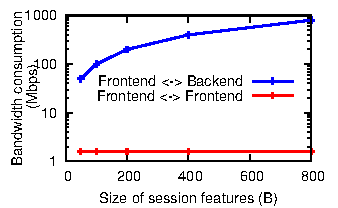
\includegraphics[width=0.45\textwidth]{figures/pytheas-Eval-bandwidth-message.pdf}
	\label{fig:eval-bandwidth-message}
}
%\hspace{-0.5cm}
\subfloat[Impact of \% sessions not in the leader cluster]
{
        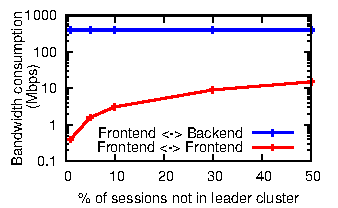
\includegraphics[width=0.45\textwidth]{figures/pytheas-Eval-bandwidth-fracproxy.pdf}
	\label{fig:eval-bandwidth-fracproxy}
}
%\hspace{-0.5cm}
%\vspace{-0.1cm}
\caption{Bandwidth consumption between clusters.}
%\vspace{-0.2cm}
\label{fig:eval-bandwidth}
\end{figure}



%\begin{figure}[t!]
%\captionsetup[subfigure]{justification=centering,farskip=-1pt,captionskip=5pt}
%\centering
%\hspace{-0.5cm}
%%\subfloat[Block-based group lookup]
%%{
%%        \includegraphics[width=0.25\textwidth]{figures/motivation/Eval-optimization-throughput-blocklookup.pdf}
%%	\label{fig:eval-optimization-throughput-blocklookup}
%%}
%%\hspace{-0.5cm}
%\subfloat[Separating logic from request responding]
%{
%        \includegraphics[width=0.25\textwidth]{figures/motivation/Eval-optimization-throughput-decoupled.pdf}
%	\label{fig:eval-optimization-throughput-decoupled}
%}
%\hspace{-0.5cm}
%\subfloat[Replacing features by group]
%{
%        \includegraphics[width=0.25\textwidth]{figures/motivation/Eval-optimization-sparkstreaming.pdf}
%	\label{fig:eval-optimization-sparkstreaming}
%}
%\hspace{-0.5cm}
%\vspace{-0.1cm}
%\tightcaption{Benefit of performance optimizations on throughput of frontend clusters.}
%%\vspace{-0.2cm}
%\label{fig:eval-bandwidth}
%\end{figure}



%Figure~\ref{fig:eval-optimization-throughput-decoupled} shows the benefit of separating logic from request responding on the throughput of  client-facing servers.
%We fixed the message size to be 100B and used one group.






\subsection{Fault Tolerance}
\label{sec:eval:fail}

Finally, we stress test the prototype under the condition that a leader frontend cluster fails. 
 We set up 10 video players, each of which can stream content from two CDNs. CDN1 has 5000ms join time and CDN2 has 1000ms join time. By default, the player's native logic chooses CDN1.
There are two frontend clusters, f1 and f2. 
The experiment begins with f1 being the leader cluster, and it loses connection at $t=25$.

Figure~\ref{fig:eval-fault-tolerance} shows the time-series of QoE of sessions that are mapped to each frontend clusters.
First, we see that the sessions mapped to f1 can fall back to the CDN chosen by the player's native logic, rather than crashing.
Second, right after f1 fails, f2 should still be able to give cached decision (made by f1 before it fails) to its sessions.
At $t=30$, the backend selects f2 as the new leader for the group. 
At the point, a naive way to restart per-group logic in the new leader is to start it from scratch, but this will lead to suboptimal QoE at the beginning (the dotted line between $t=30$ and $t=35$).
\name avoids this cold-start problem by keeping a copy of the per-group states in the proxy cluster. This allows the proxy cluster to recover the per-group control states without QoE degradation.




\begin{figure}[t!]
\centering
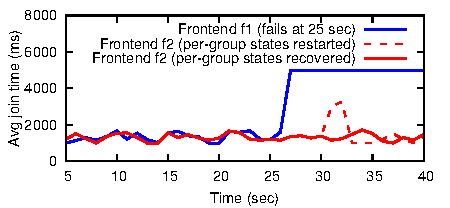
\includegraphics[width=0.6\textwidth]{figures/pytheas-Eval-fault-tolerance.pdf}
%\vspace{-0.2cm}
\caption{\name can tolerate loss of a frontend cluster by falling back to player native logic gracefully, and recovering the logic states in a new cluster.}
\label{fig:eval-fault-tolerance}
\end{figure}

